\subsection{From model information to learning from data}

The dynamic programming algorithms discussed so far rely on model information. More precisely,
they require either the transition probabilities of the MDP, or a sufficiently rich trajectory from
which the relevant quantities can be estimated.

The key question is therefore:

\begin{center}
\textbf{Can we find the optimal policy without model information?}
\end{center}

There are two different settings.

First, one may work with collected data, typically in the form of repeated episodes:
\[
(x_0,u_0,r_0),\ (x_1,u_1,r_1),\ \dots,\ (x_T,u_T,r_T).
\]
These episodes may come from repeated executions of the control task in a numerical simulator,
or from repeated experiments in a controlled environment. In this case, learning is performed
offline or between episodes: the system is allowed to generate data, and the policy is improved
using this data.

Second, one may try to learn online during the control task, with no prior training. This is
substantially harder, because the controller must learn and control at the same time:
\[
\textcolor{red}{\text{online learning}} 
\quad \Longrightarrow \quad
\text{adaptive control and dual control}.
\]
This is challenging because the input has two roles: it must achieve good performance, but it
must also excite the system enough to reveal useful information. For this reason, online
model-free optimal control is a difficult dual-control problem and, in its most general form,
comes with few guarantees.

In the following, we focus on learning methods that use data to estimate value or Q-functions.
The central idea is to replace explicit model-based policy evaluation by empirical or recursive
updates based on observed transitions.

\subsection{Monte Carlo policy evaluation}

Recall the difficult step in policy iteration. For a fixed policy \(\pi\), we would like to evaluate
the Q-function
\[
Q^\pi(x,u)
=
R_x^u
+
\gamma\sum_{x'\in\cX}P^u_{x,x'}V^\pi(x'),
\]
where
\[
V^\pi(x)
=
\E\left[
\sum_{k=0}^{\infty}\gamma^k r_k
\ \middle|\ x_0=x
\right].
\]
If the transition probabilities \(P^u_{x,x'}\) are known, this can be done by solving the
Bellman equation. In a model-free setting, instead, we try to estimate the same quantities from
observed episodes.

In Monte Carlo policy evaluation, one lets the system run under a fixed policy \(\pi\) and
records an episode
\[
(x_0,u_0,r_0),\ (x_1,u_1,r_1),\ \dots,\ (x_T,u_T,r_T).
\]
For each time \(k\), define the empirical return
\[
g_k
=
\sum_{i=k}^{T}\gamma^{i-k}r_i.
\]
This is the discounted reward accumulated from time \(k\) until the end of the episode.

The quantity \(g_k\) can be interpreted as one realization of the return associated with the
state-action pair \((x_k,u_k)\). Therefore, a basic Monte Carlo estimate is
\[
Q^\pi(x_k,u_k)\approx g_k.
\]
If the same state-action pair \((x,u)\) is visited several times, then the natural estimate is the
average of all returns observed after visits to that pair:
\[
Q^\pi(x,u)
=
\frac{
\sum_{t=0}^{T}\mathbf{1}[x_t=x,\ u_t=u]\,g_t
}{
\sum_{t=0}^{T}\mathbf{1}[x_t=x,\ u_t=u]
}.
\]
Thus, Monte Carlo policy evaluation replaces the expectation defining \(Q^\pi\) by an empirical
average over complete episodes.

\begin{figure}[h]
    \centering
    % Replace the filename below with the correct figure file.
    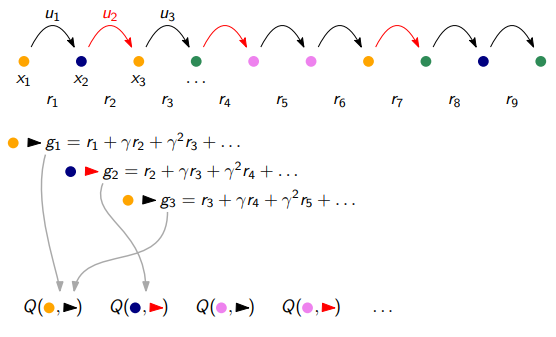
\includegraphics[width=0.85\textwidth]{images/RL_01.png}
    \caption{Monte Carlo policy evaluation. Along one episode, each visited state-action pair
    receives as target the discounted return accumulated from that time onward.}
    \label{fig:monte-carlo-policy-evaluation}
\end{figure}

The important point is that this method does not explicitly use the Bellman equation. It simply
waits until the future rewards have been observed and then computes the corresponding return.
As a consequence, the policy cannot be evaluated until the episode is over, because
\[
g_k
=
r_k+\gamma r_{k+1}+\gamma^2 r_{k+2}+\cdots
\]
depends on rewards that occur after time \(k\).

Moreover, for a finite amount of data, the resulting estimate of \(Q^\pi\) does not exactly
satisfy the Bellman equation. The Bellman equation is an identity in expectation, whereas
Monte Carlo learning is based on sample averages. Only in the limit of infinitely many
representative samples does the Monte Carlo estimate converge to the correct expected return.

This also shows a limitation of Monte Carlo learning: it does not exploit the Markov property
to make the computation more efficient. Instead of using a one-step recursive consistency
relation, it uses the full future tail of the episode.

\subsection{Temporal-difference error}

The Bellman equation for the Q-function of a fixed policy is
\[
Q^\pi(x,u)
=
R_x^u
+
\gamma\sum_{x'\in\cX}P^u_{x,x'}
\sum_{u'\in\cU}\pi(x',u')Q^\pi(x',u').
\]
Monte Carlo learning estimates \(Q^\pi\) from complete returns. Temporal-difference learning
uses a different idea: instead of waiting until the end of the episode, it uses the Bellman
equation locally, one transition at a time.

Consider one individual data point
\[
x_k,\ u_k,\ x_{k+1},\ u_{k+1},\ r_k.
\]
Given a current estimate \(Q\), define the temporal-difference error as
\[
e_k
=
r_k+\gamma Q(x_{k+1},u_{k+1})-Q(x_k,u_k).
\]
If \(Q=Q^\pi\), then the Bellman equation implies that the expected temporal-difference error
is zero:
\[
\E[e_k]=0.
\]
Thus, the TD error measures the mismatch between the current Q-value estimate and the
one-step Bellman target
\[
r_k+\gamma Q(x_{k+1},u_{k+1}).
\]
If the TD error is positive, the current estimate \(Q(x_k,u_k)\) is too small compared with the
observed one-step target. If it is negative, the current estimate is too large.

\begin{theorembox}[Temporal-difference error]
For one observed transition
\[
x_k,\ u_k,\ r_k,\ x_{k+1},\ u_{k+1},
\]
the TD error is
\[
e_k
=
r_k+\gamma Q(x_{k+1},u_{k+1})-Q(x_k,u_k).
\]
At the correct Q-function, this error has zero expectation.
\end{theorembox}

\subsection{Stochastic approximation}

Temporal-difference learning can be interpreted through stochastic approximation. Suppose we
have a random variable \(e(q)\), depending on a parameter \(q\), and we want to find a value
\(q^\star\) satisfying
\[
\E[e(q^\star)]=0.
\]
If we had access to the exact expectation, we could solve this equation directly. In learning,
however, we only observe samples of \(e(q)\). Stochastic approximation provides an iterative
method to solve such equations from noisy observations.

The basic iteration is
\[
q_{k+1}
\leftarrow
q_k-\alpha_k e(q_k).
\]
Under suitable assumptions, this converges to a solution \(q^\star\) of
\[
\E[e(q)]=0.
\]
Typical sufficient conditions are:
\begin{itemize}
    \item the random variable \(e(q)\) is bounded;
    \item the function \(\E[e(q)]\) is non-decreasing in \(q\), and increasing at \(q^\star\);
    \item the step sizes satisfy
    \[
    \sum_{k=0}^{\infty}\alpha_k=\infty,
    \qquad
    \sum_{k=0}^{\infty}\alpha_k^2<\infty.
    \]
\end{itemize}
The first condition avoids arbitrarily large noisy updates. The second condition ensures that
the expected update points toward the root. The last condition is the classical non-summable /
square-summable requirement: the steps are large enough to keep learning forever, but small
enough for the accumulated noise to remain controlled.

This viewpoint explains why temporal-difference methods update the Q-function directly from
sampled TD errors.

\subsection{TD-learning and SARSA}

TD-learning uses empirical evaluations of the temporal-difference error
\[
e_k
=
r_k+\gamma Q(x_{k+1},u_{k+1})-Q(x_k,u_k)
\]
to update the Q-function. Since the desired condition is \(\E[e_k]=0\), the Q-value associated
with the visited state-action pair is corrected in the direction of the TD error:
\[
Q(x_k,u_k)
\leftarrow
Q(x_k,u_k)
+
\alpha_k
\left(
r_k+\gamma Q(x_{k+1},u_{k+1})-Q(x_k,u_k)
\right).
\]
This algorithm is called SARSA because the update uses the quintuple
\[
(x_k,u_k,r_k,x_{k+1},u_{k+1}).
\]
The next action \(u_{k+1}\) is the action actually selected by the current policy. Therefore,
SARSA evaluates and improves the policy that is being followed.

\begin{figure}[h]
    \centering
    % Replace the filename below with the correct figure file.
    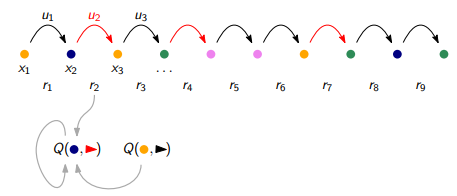
\includegraphics[width=0.85\textwidth]{images/RL_02.png}
    \caption{TD-learning with SARSA. Each observed transition immediately produces a
    one-step update of the Q-value associated with the visited state-action pair.}
    \label{fig:sarsa-td-update}
\end{figure}

Compared with Monte Carlo evaluation, the first advantage is that SARSA uses episode data
more efficiently. It does not wait until the full return \(g_k\) is available. Instead, it updates
\(Q(x_k,u_k)\) immediately after observing \(r_k\), \(x_{k+1}\), and \(u_{k+1}\).

The second important point is conceptual. SARSA enforces the Bellman equation as a
consistency principle during learning, instead of assuming that the Bellman equation will
emerge only asymptotically from complete-return averages.

If the step size \(\alpha_k\) is kept constant, the algorithm usually does not converge exactly to
a deterministic limit. Instead, it fluctuates around the solution with a steady-state nonzero
variance. Decreasing step sizes reduce this variance and are used in convergence theory.

\subsubsection{Interleaving policy evaluation and improvement}

With Monte Carlo policy iteration, one may think of alternating between:
\begin{itemize}
    \item complete policy evaluation, based on one or more full episodes;
    \item policy improvement.
\end{itemize}
Temporal-difference learning makes it possible to interleave these two operations. At every
time \(k\), one can:
\begin{enumerate}
    \item select the action \(u_k\) using the latest estimate of \(Q(x_k,u)\);
    \item observe \(r_k\), \(x_{k+1}\), and \(u_{k+1}\);
    \item update \(Q(x_k,u_k)\) using the TD rule.
\end{enumerate}

A common action-selection rule is \(\varepsilon\)-greedy:
\[
u_k
\leftarrow
\begin{cases}
\displaystyle \argmax_{u\in\cU} Q(x_k,u)
&
\text{with probability }1-\varepsilon,\\[2mm]
\text{Uniform}(\cU)
&
\text{with probability }\varepsilon.
\end{cases}
\]
The parameter \(\varepsilon\) controls exploration. During learning, one often lets
\[
\varepsilon\to 0
\qquad
\text{as}
\qquad
k\to\infty.
\]
Thus, the controller explores significantly at the beginning and becomes increasingly greedy as
the Q-function estimate improves.

In theory, this removes the need for clearly separated episodes: the policy can be improved
online as data are collected. In practice, episodic implementations remain common, but the
important conceptual step is that learning can be performed transition by transition.

\subsection{Q-learning}

SARSA uses the TD error to evaluate the current policy. Q-learning uses a closely related idea,
but applies stochastic approximation directly to the Bellman optimality equation.

The optimal Q-function satisfies
\[
Q^\star(x,u)
=
R_x^u
+
\gamma\sum_{x'\in\cX}P^u_{x,x'}
\left(
\max_{u'\in\cU}Q^\star(x',u')
\right).
\]
For an individual transition, the corresponding sample realization of the Bellman optimality
target is
\[
r_k+\gamma\max_{u'\in\cU}Q(x_{k+1},u').
\]
Therefore, the Q-learning update is
\[
Q(x_k,u_k)
\leftarrow
Q(x_k,u_k)
+
\alpha_k
\left(
r_k
+
\gamma\max_{u'\in\cU}Q(x_{k+1},u')
-
Q(x_k,u_k)
\right).
\]
This is the same temporal-difference structure as SARSA, but with a crucial difference: the next
action used in the update is not the action actually taken by the policy. Instead, the update uses
the greedy value
\[
\max_{u'\in\cU}Q(x_{k+1},u').
\]
For this reason, Q-learning is an \textbf{off-policy} algorithm.

\begin{theorembox}[Q-learning update]
For an observed transition
\[
x_k,\ u_k,\ r_k,\ x_{k+1},
\]
the Q-learning update is
\[
Q(x_k,u_k)
\leftarrow
Q(x_k,u_k)
+
\alpha_k
\left(
r_k
+
\gamma\max_{u'\in\cU}Q(x_{k+1},u')
-
Q(x_k,u_k)
\right).
\]
\end{theorembox}

There are several important points to notice.

First, the input \(u_{k+1}\) is irrelevant for the update. The action actually selected at the next
state does not need to be optimal, because the update assumes optimal future play through the
maximum over \(u'\).

Second, convergence to the optimal Q-function is guaranteed under classical assumptions such
as sufficient exploration of all state-action pairs and suitable step sizes satisfying the
non-summable / square-summable conditions.

Third, the policy is typically updated as \(\varepsilon\)-greedy. Even though the learning update
is off-policy, exploration is still needed in order to visit the state-action space. In practice, it is
often useful to explore more actions at the beginning and then gradually concentrate exploration
around high-reward actions.

Finally, Q-learning can be interpreted as a forward version of dynamic programming. Instead
of sweeping over all states using a known model, it updates the Q-function along the trajectory
generated by interaction with the system.

\subsection{SARSA versus Q-learning}

The main difference between SARSA and Q-learning is the following:
\[
\text{SARSA learns on-policy,}
\qquad
\text{Q-learning learns off-policy.}
\]

SARSA evaluates the policy that is actually being used. The update contains
\[
Q(x_{k+1},u_{k+1}),
\]
where \(u_{k+1}\) is the action selected by the current, possibly exploratory, policy. Therefore,
SARSA takes into account the fact that future actions may still include exploration.

Q-learning instead uses
\[
\max_{u'\in\cU}Q(x_{k+1},u'),
\]
independently of which action will actually be taken next. Hence it learns the optimal Q-function
associated with greedy future behavior, even while the data are generated by an exploratory
policy.

This makes SARSA more conservative. Since it learns the value of the exploratory policy, it
accounts for the residual exploration that will occur in the future. Q-learning is more aggressive:
it assumes optimal future action selection and therefore pushes the policy toward the optimal
greedy strategy more directly.

In reward maximization, once the optimal Q-function has been learned, the optimal policy is
obtained by extracting
\[
\mu^\star(x)
\in
\argmax_{u\in\cU}Q^\star(x,u).
\]

\subsection{Q-learning as stochastic gradient descent}

The Q-learning update can also be interpreted as a stochastic gradient step for minimizing the
error in the Bellman optimality principle.

Consider the Bellman optimality residual for a state-action pair \((x,u)\):
\[
R_x^u
+
\gamma\sum_{x'\in\cX}P^u_{x,x'}
\max_{u'\in\cU}Q(x',u')
-
Q(x,u).
\]
A natural loss function is
\[
\mathcal{L}
=
\frac{1}{2}
\left(
R_x^u
+
\gamma\sum_{x'\in\cX}P^u_{x,x'}
\max_{u'\in\cU}Q(x',u')
-
\textcolor{red}{Q(x,u)}
\right)^2.
\]
Here the current estimate of \(Q(x',u')\) is used inside the target. This is called
\textbf{bootstrapping}: the target itself depends on the current value function estimate.

If we differentiate the loss with respect to the decision variable \(Q(x,u)\), treating the target
as fixed, we obtain
\[
\nabla_{Q(x,u)}\mathcal{L}
=
-
\left(
R_x^u
+
\gamma\sum_{x'\in\cX}P^u_{x,x'}
\max_{u'\in\cU}Q(x',u')
-
Q(x,u)
\right).
\]
The model-free sample version of this gradient is
\[
-
\left(
r_k
+
\gamma\max_{u'\in\cU}Q(x_{k+1},u')
-
Q(x_k,u_k)
\right).
\]
A stochastic gradient descent step therefore gives exactly the Q-learning update:
\[
Q(x_k,u_k)
\leftarrow
Q(x_k,u_k)
+
\alpha_k
\left(
r_k
+
\gamma\max_{u'\in\cU}Q(x_{k+1},u')
-
Q(x_k,u_k)
\right).
\]
Thus, Q-learning can be viewed as stochastic gradient descent on the Bellman optimality error.

\subsection{Q-learning with linear approximation}

For large state-action spaces, a tabular representation of \(Q(x,u)\) is not scalable. As before,
we introduce a linear parametrization
\[
Q_\theta(x,u)
=
\sum_{\ell=1}^{d}\phi_\ell(x,u)\theta_\ell
=
\phi(x,u)^\top\theta.
\]
The goal is now to update the parameter vector \(\theta\) so that \(Q_\theta\) approximately
satisfies the Bellman optimality principle
\[
Q^\star(x,u)
=
R_x^u
+
\gamma\sum_{x'\in\cX}P^u_{x,x'}
\left(
\max_{u'\in\cU}Q^\star(x',u')
\right).
\]
In terms of the parametrization, this would require
\[
\phi(x,u)^\top\theta^\star
=
R_x^u
+
\gamma\sum_{x'\in\cX}P^u_{x,x'}
\left(
\max_{u'\in\cU}\phi(x',u')^\top\theta^\star
\right).
\]
In general, this equation does not have an exact solution in the chosen function class. The
parametrization may be too restrictive, so no parameter vector \(\theta\) may satisfy the
Bellman optimality equation for all state-action pairs simultaneously.

For a fixed sample, define the target
\[
Q^+
=
R_x^u
+
\gamma\sum_{x'\in\cX}P^u_{x,x'}
\left(
\max_{u'\in\cU}\phi(x',u')^\top\theta
\right).
\]
Then a least-squares loss for the current state-action pair is
\[
\min_{\theta}
\frac{1}{2}
\left(
\phi(x,u)^\top\theta-Q^+
\right)^2.
\]
The corresponding gradient descent iteration is
\[
\theta_{k+1}
=
\theta_k
-
\alpha
\left(
\phi(x,u)^\top\theta_k-Q^+
\right)\phi(x,u).
\]

In a model-free setting, we do not know the expectation defining \(Q^+\). We replace it by the
sampled target
\[
r_k
+
\gamma\max_{u\in\cU}\phi(x_{k+1},u)^\top\theta_k.
\]
This gives the stochastic gradient update
\[
\theta_{k+1}
=
\theta_k
-
\alpha_k
\left(
\phi(x_k,u_k)^\top\theta_k
-
\left(
r_k+\gamma\max_{u\in\cU}\phi(x_{k+1},u)^\top\theta_k
\right)
\right)
\phi(x_k,u_k).
\]
Equivalently,
\[
\theta_{k+1}
=
\theta_k
+
\alpha_k
\left(
r_k+\gamma\max_{u\in\cU}Q_{\theta_k}(x_{k+1},u)
-
Q_{\theta_k}(x_k,u_k)
\right)
\phi(x_k,u_k).
\]
This is Q-learning with a linear approximator.

\subsection{General approximators}

Linear parametrizations are useful because they are simple and transparent, but more complex
function approximators can also be used. For instance, one can represent the Q-function by a
neural network
\[
Q_\theta(x,u),
\]
where \(\theta\) collects all the weights of the network.\\
The requirements are conceptually the same:
\begin{itemize}
    \item the approximator must provide a parametrized function \(Q_\theta(x,u)\);
    \item it must be possible to compute or approximate
    \[
    \max_{u\in\cU}Q_\theta(x,u);
    \]
    \item it must be possible to perform a stochastic gradient step in \(\theta\) to reduce a
    Bellman-error loss.
\end{itemize}
For neural networks, the gradient step is computed by backpropagation. The resulting methods
are the basis of deep Q-learning and related algorithms.

\subsection{Is it really model-free?}

Monte Carlo and temporal-difference methods seem to avoid the need for a model of the
system. They do not require explicit transition probabilities \(P^u_{x,x'}\), and they can update
the value or Q-function directly from sampled data.

However, there is still implicit structure. In particular, these methods assume that the process
admits a Markovian state \(x\). The Q-function
\[
Q(x,u)
\]
is meaningful only if \(x\) contains all information needed to predict the future distribution of
rewards after choosing action \(u\). Thus, even if the transition probabilities are not known, we
are still assuming that the chosen state representation is Markovian.

This raises a further question: is it possible to learn the policy directly, without first learning
a value function or Q-function? This leads to policy-gradient methods.

\subsection{Policy gradient methods}

Instead of representing a value function, policy-gradient methods directly parametrize the
policy. Consider a trajectory of the system
\[
\tau
=
(x_0,u_0,x_1,u_1,\dots,x_T,u_T,x_{T+1}).
\]
For simplicity, assume that the initial state \(x_0\) is fixed across episodes.

The reward associated with the trajectory is
\[
R(\tau)
=
\sum_{t=0}^{T}\gamma^t r_t.
\]
We now introduce a stochastic policy parametrized by a vector \(\theta\):
\[
\pi_\theta(x,u).
\]
The parametrization may be:
\begin{itemize}
    \item based on a linear combination of features \(\phi(x,u)^\top\theta\);
    \item based on a parametric distribution, such as a Gaussian policy;
    \item based on a neural network with weights \(\theta\).
\end{itemize}

The goal is to maximize the expected reward
\[
J(\theta)
=
\E_{\tau\sim\pi_\theta}[R(\tau)].
\]
Equivalently,
\[
J(\theta)
=
\sum_{\tau}\Prob_\theta(\tau)R(\tau),
\]
where \(\Prob_\theta(\tau)\) is the probability that the trajectory \(\tau\) occurs when the policy
\(\pi_\theta\) is used.

There are two sources of complexity:
\begin{enumerate}
    \item \(J(\theta)\) is an expectation, hence it involves a sum over all possible trajectories;
    \item \(\Prob_\theta(\tau)\) is unknown, because it depends both on the system transition
    probabilities and on the policy.
\end{enumerate}

The probability of a trajectory can be factorized as
\[
\Prob_\theta(\tau)
=
\prod_{t=0}^{T}
\underbrace{\Prob(x_{t+1}\mid x_t,u_t)}_{\text{transition probabilities}}
\underbrace{\pi_\theta(x_t,u_t)}_{\text{policy}}.
\]
This expression separates the two mechanisms that generate a trajectory. The environment
determines the next state through the transition probabilities, while the controller determines
the action through the policy.

The central idea of policy-gradient methods is to optimize \(J(\theta)\) directly, using sampled
trajectories to estimate the gradient with respect to \(\theta\). The derivation of such estimators
starts from the trajectory-probability factorization above.